\documentclass[border=5pt]{standalone}
\usepackage[T1]{fontenc}\usepackage{lmodern}\usepackage{pgfplots}
\pgfplotsset{compat=1.18}\begin{document}\sffamily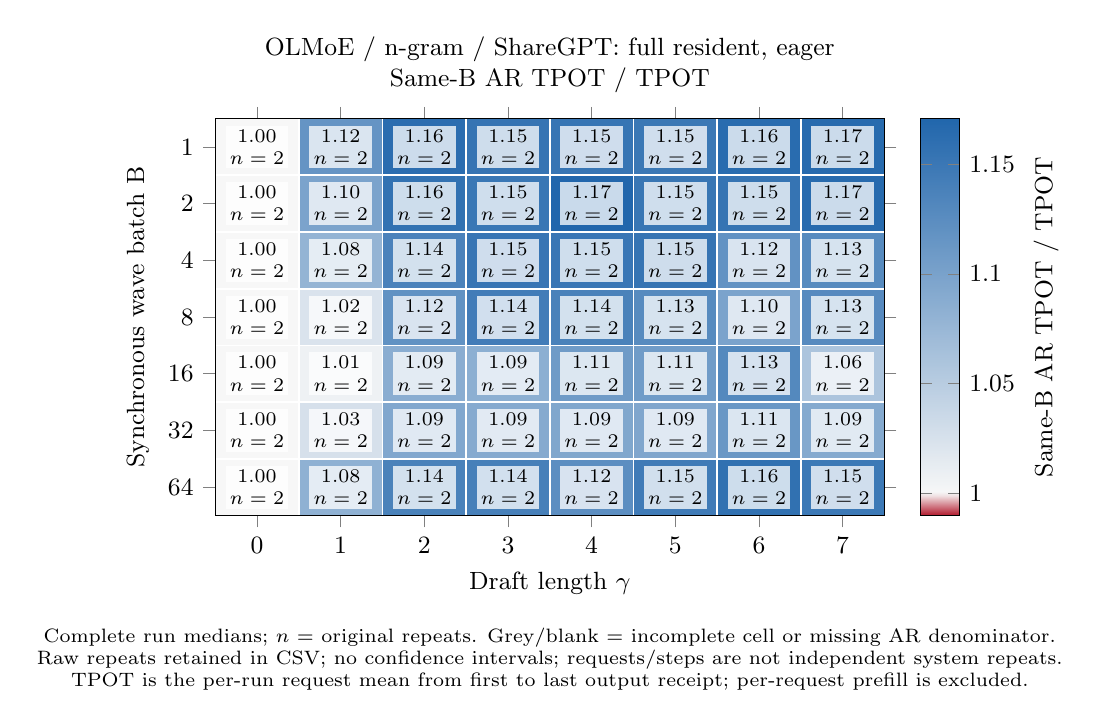
\begin{tikzpicture}
\begin{axis}[name=matrix,width=8.50cm,height=5.04cm,scale only axis,xmin=-.5,xmax=7.5,ymin=-.5,ymax=6.5,y dir=reverse,axis on top,tick align=outside,xtick={0,1,2,3,4,5,6,7},xticklabels={0,1,2,3,4,5,6,7},ytick={0,1,2,3,4,5,6},yticklabels={1,2,4,8,16,32,64},xlabel={Draft length $\gamma$},ylabel={Synchronous wave batch B},title={OLMoE / n-gram / ShareGPT: full resident, eager\\Same-B AR TPOT / TPOT},title style={align=center,font=\small},tick label style={font=\small},label style={font=\small},point meta min=0.99,point meta max=1.17067768388,colormap={matrixcolors}{rgb255=(178,24,43); rgb255=(190,64,80); rgb255=(203,105,117); rgb255=(215,145,154); rgb255=(228,185,190); rgb255=(240,225,227); rgb255=(246,246,247); rgb255=(244,245,246); rgb255=(241,243,245); rgb255=(239,242,244); rgb255=(237,240,243); rgb255=(235,239,243); rgb255=(232,237,242); rgb255=(230,236,241); rgb255=(228,234,240); rgb255=(226,232,239); rgb255=(223,231,239); rgb255=(221,229,238); rgb255=(219,228,237); rgb255=(216,226,236); rgb255=(214,225,236); rgb255=(212,223,235); rgb255=(210,222,234); rgb255=(207,220,233); rgb255=(205,219,232); rgb255=(203,217,232); rgb255=(201,216,231); rgb255=(198,214,230); rgb255=(196,213,229); rgb255=(194,211,228); rgb255=(192,209,228); rgb255=(189,208,227); rgb255=(187,206,226); rgb255=(185,205,225); rgb255=(183,203,224); rgb255=(180,202,224); rgb255=(178,200,223); rgb255=(176,199,222); rgb255=(173,197,221); rgb255=(171,196,220); rgb255=(169,194,220); rgb255=(167,193,219); rgb255=(164,191,218); rgb255=(162,189,217); rgb255=(160,188,216); rgb255=(158,186,216); rgb255=(155,185,215); rgb255=(153,183,214); rgb255=(151,182,213); rgb255=(149,180,212); rgb255=(146,179,212); rgb255=(144,177,211); rgb255=(142,176,210); rgb255=(139,174,209); rgb255=(137,173,209); rgb255=(135,171,208); rgb255=(133,170,207); rgb255=(130,168,206); rgb255=(128,166,205); rgb255=(126,165,205); rgb255=(124,163,204); rgb255=(121,162,203); rgb255=(119,160,202); rgb255=(117,159,201); rgb255=(115,157,201); rgb255=(112,156,200); rgb255=(110,154,199); rgb255=(108,153,198); rgb255=(105,151,197); rgb255=(103,150,197); rgb255=(101,148,196); rgb255=(99,147,195); rgb255=(96,145,194); rgb255=(94,143,193); rgb255=(92,142,193); rgb255=(90,140,192); rgb255=(87,139,191); rgb255=(85,137,190); rgb255=(83,136,189); rgb255=(81,134,189); rgb255=(78,133,188); rgb255=(76,131,187); rgb255=(74,130,186); rgb255=(72,128,185); rgb255=(69,127,185); rgb255=(67,125,184); rgb255=(65,123,183); rgb255=(62,122,182); rgb255=(60,120,182); rgb255=(58,119,181); rgb255=(56,117,180); rgb255=(53,116,179); rgb255=(51,114,178); rgb255=(49,113,178); rgb255=(47,111,177); rgb255=(44,110,176); rgb255=(42,108,175); rgb255=(40,107,174); rgb255=(38,105,174); rgb255=(35,104,173); rgb255=(33,102,172)},colorbar,colorbar style={ylabel={Same-B AR TPOT / TPOT},label style={font=\small},tick label style={font=\small}}]
\path[fill={rgb,255:red,247;green,247;blue,247},draw=white,line width=.6pt] (axis cs:-0.5,-0.5) rectangle (axis cs:0.5,0.5);
\node[align=center,font=\scriptsize,fill=white,fill opacity=.76,text opacity=1,inner sep=1.5pt] at (axis cs:0,0) {1.00\\$n=2$};
\path[fill={rgb,255:red,101;green,148;blue,196},draw=white,line width=.6pt] (axis cs:0.5,-0.5) rectangle (axis cs:1.5,0.5);
\node[align=center,font=\scriptsize,fill=white,fill opacity=.76,text opacity=1,inner sep=1.5pt] at (axis cs:1,0) {1.12\\$n=2$};
\path[fill={rgb,255:red,43;green,109;blue,176},draw=white,line width=.6pt] (axis cs:1.5,-0.5) rectangle (axis cs:2.5,0.5);
\node[align=center,font=\scriptsize,fill=white,fill opacity=.76,text opacity=1,inner sep=1.5pt] at (axis cs:2,0) {1.16\\$n=2$};
\path[fill={rgb,255:red,54;green,116;blue,179},draw=white,line width=.6pt] (axis cs:2.5,-0.5) rectangle (axis cs:3.5,0.5);
\node[align=center,font=\scriptsize,fill=white,fill opacity=.76,text opacity=1,inner sep=1.5pt] at (axis cs:3,0) {1.15\\$n=2$};
\path[fill={rgb,255:red,55;green,117;blue,180},draw=white,line width=.6pt] (axis cs:3.5,-0.5) rectangle (axis cs:4.5,0.5);
\node[align=center,font=\scriptsize,fill=white,fill opacity=.76,text opacity=1,inner sep=1.5pt] at (axis cs:4,0) {1.15\\$n=2$};
\path[fill={rgb,255:red,59;green,120;blue,181},draw=white,line width=.6pt] (axis cs:4.5,-0.5) rectangle (axis cs:5.5,0.5);
\node[align=center,font=\scriptsize,fill=white,fill opacity=.76,text opacity=1,inner sep=1.5pt] at (axis cs:5,0) {1.15\\$n=2$};
\path[fill={rgb,255:red,41;green,108;blue,175},draw=white,line width=.6pt] (axis cs:5.5,-0.5) rectangle (axis cs:6.5,0.5);
\node[align=center,font=\scriptsize,fill=white,fill opacity=.76,text opacity=1,inner sep=1.5pt] at (axis cs:6,0) {1.16\\$n=2$};
\path[fill={rgb,255:red,40;green,107;blue,174},draw=white,line width=.6pt] (axis cs:6.5,-0.5) rectangle (axis cs:7.5,0.5);
\node[align=center,font=\scriptsize,fill=white,fill opacity=.76,text opacity=1,inner sep=1.5pt] at (axis cs:7,0) {1.17\\$n=2$};
\path[fill={rgb,255:red,247;green,247;blue,247},draw=white,line width=.6pt] (axis cs:-0.5,0.5) rectangle (axis cs:0.5,1.5);
\node[align=center,font=\scriptsize,fill=white,fill opacity=.76,text opacity=1,inner sep=1.5pt] at (axis cs:0,1) {1.00\\$n=2$};
\path[fill={rgb,255:red,123;green,163;blue,204},draw=white,line width=.6pt] (axis cs:0.5,0.5) rectangle (axis cs:1.5,1.5);
\node[align=center,font=\scriptsize,fill=white,fill opacity=.76,text opacity=1,inner sep=1.5pt] at (axis cs:1,1) {1.10\\$n=2$};
\path[fill={rgb,255:red,50;green,114;blue,178},draw=white,line width=.6pt] (axis cs:1.5,0.5) rectangle (axis cs:2.5,1.5);
\node[align=center,font=\scriptsize,fill=white,fill opacity=.76,text opacity=1,inner sep=1.5pt] at (axis cs:2,1) {1.16\\$n=2$};
\path[fill={rgb,255:red,57;green,119;blue,181},draw=white,line width=.6pt] (axis cs:2.5,0.5) rectangle (axis cs:3.5,1.5);
\node[align=center,font=\scriptsize,fill=white,fill opacity=.76,text opacity=1,inner sep=1.5pt] at (axis cs:3,1) {1.15\\$n=2$};
\path[fill={rgb,255:red,33;green,102;blue,172},draw=white,line width=.6pt] (axis cs:3.5,0.5) rectangle (axis cs:4.5,1.5);
\node[align=center,font=\scriptsize,fill=white,fill opacity=.76,text opacity=1,inner sep=1.5pt] at (axis cs:4,1) {1.17\\$n=2$};
\path[fill={rgb,255:red,56;green,118;blue,180},draw=white,line width=.6pt] (axis cs:4.5,0.5) rectangle (axis cs:5.5,1.5);
\node[align=center,font=\scriptsize,fill=white,fill opacity=.76,text opacity=1,inner sep=1.5pt] at (axis cs:5,1) {1.15\\$n=2$};
\path[fill={rgb,255:red,54;green,116;blue,179},draw=white,line width=.6pt] (axis cs:5.5,0.5) rectangle (axis cs:6.5,1.5);
\node[align=center,font=\scriptsize,fill=white,fill opacity=.76,text opacity=1,inner sep=1.5pt] at (axis cs:6,1) {1.15\\$n=2$};
\path[fill={rgb,255:red,40;green,107;blue,174},draw=white,line width=.6pt] (axis cs:6.5,0.5) rectangle (axis cs:7.5,1.5);
\node[align=center,font=\scriptsize,fill=white,fill opacity=.76,text opacity=1,inner sep=1.5pt] at (axis cs:7,1) {1.17\\$n=2$};
\path[fill={rgb,255:red,247;green,247;blue,247},draw=white,line width=.6pt] (axis cs:-0.5,1.5) rectangle (axis cs:0.5,2.5);
\node[align=center,font=\scriptsize,fill=white,fill opacity=.76,text opacity=1,inner sep=1.5pt] at (axis cs:0,2) {1.00\\$n=2$};
\path[fill={rgb,255:red,148;green,180;blue,212},draw=white,line width=.6pt] (axis cs:0.5,1.5) rectangle (axis cs:1.5,2.5);
\node[align=center,font=\scriptsize,fill=white,fill opacity=.76,text opacity=1,inner sep=1.5pt] at (axis cs:1,2) {1.08\\$n=2$};
\path[fill={rgb,255:red,75;green,130;blue,187},draw=white,line width=.6pt] (axis cs:1.5,1.5) rectangle (axis cs:2.5,2.5);
\node[align=center,font=\scriptsize,fill=white,fill opacity=.76,text opacity=1,inner sep=1.5pt] at (axis cs:2,2) {1.14\\$n=2$};
\path[fill={rgb,255:red,56;green,117;blue,180},draw=white,line width=.6pt] (axis cs:2.5,1.5) rectangle (axis cs:3.5,2.5);
\node[align=center,font=\scriptsize,fill=white,fill opacity=.76,text opacity=1,inner sep=1.5pt] at (axis cs:3,2) {1.15\\$n=2$};
\path[fill={rgb,255:red,57;green,118;blue,181},draw=white,line width=.6pt] (axis cs:3.5,1.5) rectangle (axis cs:4.5,2.5);
\node[align=center,font=\scriptsize,fill=white,fill opacity=.76,text opacity=1,inner sep=1.5pt] at (axis cs:4,2) {1.15\\$n=2$};
\path[fill={rgb,255:red,54;green,116;blue,179},draw=white,line width=.6pt] (axis cs:4.5,1.5) rectangle (axis cs:5.5,2.5);
\node[align=center,font=\scriptsize,fill=white,fill opacity=.76,text opacity=1,inner sep=1.5pt] at (axis cs:5,2) {1.15\\$n=2$};
\path[fill={rgb,255:red,98;green,146;blue,195},draw=white,line width=.6pt] (axis cs:5.5,1.5) rectangle (axis cs:6.5,2.5);
\node[align=center,font=\scriptsize,fill=white,fill opacity=.76,text opacity=1,inner sep=1.5pt] at (axis cs:6,2) {1.12\\$n=2$};
\path[fill={rgb,255:red,87;green,139;blue,191},draw=white,line width=.6pt] (axis cs:6.5,1.5) rectangle (axis cs:7.5,2.5);
\node[align=center,font=\scriptsize,fill=white,fill opacity=.76,text opacity=1,inner sep=1.5pt] at (axis cs:7,2) {1.13\\$n=2$};
\path[fill={rgb,255:red,247;green,247;blue,247},draw=white,line width=.6pt] (axis cs:-0.5,2.5) rectangle (axis cs:0.5,3.5);
\node[align=center,font=\scriptsize,fill=white,fill opacity=.76,text opacity=1,inner sep=1.5pt] at (axis cs:0,3) {1.00\\$n=2$};
\path[fill={rgb,255:red,218;green,227;blue,237},draw=white,line width=.6pt] (axis cs:0.5,2.5) rectangle (axis cs:1.5,3.5);
\node[align=center,font=\scriptsize,fill=white,fill opacity=.76,text opacity=1,inner sep=1.5pt] at (axis cs:1,3) {1.02\\$n=2$};
\path[fill={rgb,255:red,97;green,146;blue,195},draw=white,line width=.6pt] (axis cs:1.5,2.5) rectangle (axis cs:2.5,3.5);
\node[align=center,font=\scriptsize,fill=white,fill opacity=.76,text opacity=1,inner sep=1.5pt] at (axis cs:2,3) {1.12\\$n=2$};
\path[fill={rgb,255:red,66;green,124;blue,184},draw=white,line width=.6pt] (axis cs:2.5,2.5) rectangle (axis cs:3.5,3.5);
\node[align=center,font=\scriptsize,fill=white,fill opacity=.76,text opacity=1,inner sep=1.5pt] at (axis cs:3,3) {1.14\\$n=2$};
\path[fill={rgb,255:red,74;green,130;blue,186},draw=white,line width=.6pt] (axis cs:3.5,2.5) rectangle (axis cs:4.5,3.5);
\node[align=center,font=\scriptsize,fill=white,fill opacity=.76,text opacity=1,inner sep=1.5pt] at (axis cs:4,3) {1.14\\$n=2$};
\path[fill={rgb,255:red,87;green,139;blue,191},draw=white,line width=.6pt] (axis cs:4.5,2.5) rectangle (axis cs:5.5,3.5);
\node[align=center,font=\scriptsize,fill=white,fill opacity=.76,text opacity=1,inner sep=1.5pt] at (axis cs:5,3) {1.13\\$n=2$};
\path[fill={rgb,255:red,123;green,163;blue,204},draw=white,line width=.6pt] (axis cs:5.5,2.5) rectangle (axis cs:6.5,3.5);
\node[align=center,font=\scriptsize,fill=white,fill opacity=.76,text opacity=1,inner sep=1.5pt] at (axis cs:6,3) {1.10\\$n=2$};
\path[fill={rgb,255:red,87;green,138;blue,191},draw=white,line width=.6pt] (axis cs:6.5,2.5) rectangle (axis cs:7.5,3.5);
\node[align=center,font=\scriptsize,fill=white,fill opacity=.76,text opacity=1,inner sep=1.5pt] at (axis cs:7,3) {1.13\\$n=2$};
\path[fill={rgb,255:red,247;green,247;blue,247},draw=white,line width=.6pt] (axis cs:-0.5,3.5) rectangle (axis cs:0.5,4.5);
\node[align=center,font=\scriptsize,fill=white,fill opacity=.76,text opacity=1,inner sep=1.5pt] at (axis cs:0,4) {1.00\\$n=2$};
\path[fill={rgb,255:red,238;green,241;blue,244},draw=white,line width=.6pt] (axis cs:0.5,3.5) rectangle (axis cs:1.5,4.5);
\node[align=center,font=\scriptsize,fill=white,fill opacity=.76,text opacity=1,inner sep=1.5pt] at (axis cs:1,4) {1.01\\$n=2$};
\path[fill={rgb,255:red,138;green,173;blue,209},draw=white,line width=.6pt] (axis cs:1.5,3.5) rectangle (axis cs:2.5,4.5);
\node[align=center,font=\scriptsize,fill=white,fill opacity=.76,text opacity=1,inner sep=1.5pt] at (axis cs:2,4) {1.09\\$n=2$};
\path[fill={rgb,255:red,140;green,175;blue,210},draw=white,line width=.6pt] (axis cs:2.5,3.5) rectangle (axis cs:3.5,4.5);
\node[align=center,font=\scriptsize,fill=white,fill opacity=.76,text opacity=1,inner sep=1.5pt] at (axis cs:3,4) {1.09\\$n=2$};
\path[fill={rgb,255:red,111;green,155;blue,199},draw=white,line width=.6pt] (axis cs:3.5,3.5) rectangle (axis cs:4.5,4.5);
\node[align=center,font=\scriptsize,fill=white,fill opacity=.76,text opacity=1,inner sep=1.5pt] at (axis cs:4,4) {1.11\\$n=2$};
\path[fill={rgb,255:red,112;green,156;blue,200},draw=white,line width=.6pt] (axis cs:4.5,3.5) rectangle (axis cs:5.5,4.5);
\node[align=center,font=\scriptsize,fill=white,fill opacity=.76,text opacity=1,inner sep=1.5pt] at (axis cs:5,4) {1.11\\$n=2$};
\path[fill={rgb,255:red,84;green,137;blue,190},draw=white,line width=.6pt] (axis cs:5.5,3.5) rectangle (axis cs:6.5,4.5);
\node[align=center,font=\scriptsize,fill=white,fill opacity=.76,text opacity=1,inner sep=1.5pt] at (axis cs:6,4) {1.13\\$n=2$};
\path[fill={rgb,255:red,172;green,196;blue,221},draw=white,line width=.6pt] (axis cs:6.5,3.5) rectangle (axis cs:7.5,4.5);
\node[align=center,font=\scriptsize,fill=white,fill opacity=.76,text opacity=1,inner sep=1.5pt] at (axis cs:7,4) {1.06\\$n=2$};
\path[fill={rgb,255:red,247;green,247;blue,247},draw=white,line width=.6pt] (axis cs:-0.5,4.5) rectangle (axis cs:0.5,5.5);
\node[align=center,font=\scriptsize,fill=white,fill opacity=.76,text opacity=1,inner sep=1.5pt] at (axis cs:0,5) {1.00\\$n=2$};
\path[fill={rgb,255:red,214;green,224;blue,235},draw=white,line width=.6pt] (axis cs:0.5,4.5) rectangle (axis cs:1.5,5.5);
\node[align=center,font=\scriptsize,fill=white,fill opacity=.76,text opacity=1,inner sep=1.5pt] at (axis cs:1,5) {1.03\\$n=2$};
\path[fill={rgb,255:red,129;green,167;blue,206},draw=white,line width=.6pt] (axis cs:1.5,4.5) rectangle (axis cs:2.5,5.5);
\node[align=center,font=\scriptsize,fill=white,fill opacity=.76,text opacity=1,inner sep=1.5pt] at (axis cs:2,5) {1.09\\$n=2$};
\path[fill={rgb,255:red,134;green,170;blue,207},draw=white,line width=.6pt] (axis cs:2.5,4.5) rectangle (axis cs:3.5,5.5);
\node[align=center,font=\scriptsize,fill=white,fill opacity=.76,text opacity=1,inner sep=1.5pt] at (axis cs:3,5) {1.09\\$n=2$};
\path[fill={rgb,255:red,128;green,167;blue,205},draw=white,line width=.6pt] (axis cs:3.5,4.5) rectangle (axis cs:4.5,5.5);
\node[align=center,font=\scriptsize,fill=white,fill opacity=.76,text opacity=1,inner sep=1.5pt] at (axis cs:4,5) {1.09\\$n=2$};
\path[fill={rgb,255:red,128;green,166;blue,205},draw=white,line width=.6pt] (axis cs:4.5,4.5) rectangle (axis cs:5.5,5.5);
\node[align=center,font=\scriptsize,fill=white,fill opacity=.76,text opacity=1,inner sep=1.5pt] at (axis cs:5,5) {1.09\\$n=2$};
\path[fill={rgb,255:red,105;green,151;blue,197},draw=white,line width=.6pt] (axis cs:5.5,4.5) rectangle (axis cs:6.5,5.5);
\node[align=center,font=\scriptsize,fill=white,fill opacity=.76,text opacity=1,inner sep=1.5pt] at (axis cs:6,5) {1.11\\$n=2$};
\path[fill={rgb,255:red,133;green,170;blue,207},draw=white,line width=.6pt] (axis cs:6.5,4.5) rectangle (axis cs:7.5,5.5);
\node[align=center,font=\scriptsize,fill=white,fill opacity=.76,text opacity=1,inner sep=1.5pt] at (axis cs:7,5) {1.09\\$n=2$};
\path[fill={rgb,255:red,247;green,247;blue,247},draw=white,line width=.6pt] (axis cs:-0.5,5.5) rectangle (axis cs:0.5,6.5);
\node[align=center,font=\scriptsize,fill=white,fill opacity=.76,text opacity=1,inner sep=1.5pt] at (axis cs:0,6) {1.00\\$n=2$};
\path[fill={rgb,255:red,143;green,177;blue,211},draw=white,line width=.6pt] (axis cs:0.5,5.5) rectangle (axis cs:1.5,6.5);
\node[align=center,font=\scriptsize,fill=white,fill opacity=.76,text opacity=1,inner sep=1.5pt] at (axis cs:1,6) {1.08\\$n=2$};
\path[fill={rgb,255:red,74;green,130;blue,186},draw=white,line width=.6pt] (axis cs:1.5,5.5) rectangle (axis cs:2.5,6.5);
\node[align=center,font=\scriptsize,fill=white,fill opacity=.76,text opacity=1,inner sep=1.5pt] at (axis cs:2,6) {1.14\\$n=2$};
\path[fill={rgb,255:red,71;green,128;blue,185},draw=white,line width=.6pt] (axis cs:2.5,5.5) rectangle (axis cs:3.5,6.5);
\node[align=center,font=\scriptsize,fill=white,fill opacity=.76,text opacity=1,inner sep=1.5pt] at (axis cs:3,6) {1.14\\$n=2$};
\path[fill={rgb,255:red,92;green,142;blue,193},draw=white,line width=.6pt] (axis cs:3.5,5.5) rectangle (axis cs:4.5,6.5);
\node[align=center,font=\scriptsize,fill=white,fill opacity=.76,text opacity=1,inner sep=1.5pt] at (axis cs:4,6) {1.12\\$n=2$};
\path[fill={rgb,255:red,64;green,123;blue,183},draw=white,line width=.6pt] (axis cs:4.5,5.5) rectangle (axis cs:5.5,6.5);
\node[align=center,font=\scriptsize,fill=white,fill opacity=.76,text opacity=1,inner sep=1.5pt] at (axis cs:5,6) {1.15\\$n=2$};
\path[fill={rgb,255:red,49;green,113;blue,177},draw=white,line width=.6pt] (axis cs:5.5,5.5) rectangle (axis cs:6.5,6.5);
\node[align=center,font=\scriptsize,fill=white,fill opacity=.76,text opacity=1,inner sep=1.5pt] at (axis cs:6,6) {1.16\\$n=2$};
\path[fill={rgb,255:red,60;green,121;blue,182},draw=white,line width=.6pt] (axis cs:6.5,5.5) rectangle (axis cs:7.5,6.5);
\node[align=center,font=\scriptsize,fill=white,fill opacity=.76,text opacity=1,inner sep=1.5pt] at (axis cs:7,6) {1.15\\$n=2$};
\end{axis}
\node[below=1.3cm,align=center,font=\scriptsize] at (matrix.south) {Complete run medians; $n$ = original repeats. Grey/blank = incomplete cell or missing AR denominator.\\Raw repeats retained in CSV; no confidence intervals; requests/steps are not independent system repeats.\\TPOT is the per-run request mean from first to last output receipt; per-request prefill is excluded.};
\end{tikzpicture}\end{document}
